\chapter{Hand-Crated LL(k) Parser}
\textbf{Note: } Production rules of tinylang’s EBNF as stated
in section \ref{sec:ebnf-tinylang-rules} avoids left recursion. This avoids the problem of having recursive descent parser to loop indefinitely.
\section{The parser}
A tinylang program is parsed using a hand-crafted predictive top-down
parser.
Features of the parser:
\begin{itemize}
	\item \textbf{Top-down parsing.} Top-down parsing in computer science is a parsing strategy where one first looks at the highest level of the parse tree and works down the abstract syntax tree by using the rewriting rules of a formal grammar until we reach the leaves.
	\item  \textbf{Recursive Descent.} The procedures required to move down the abstract syntax tree correspond to one of the non-terminal symbols of the grammar.
	\item \textbf{k=1.} 1 look-ahead token is enough to choose which production rule to use. This allows the parser to be efficient since it is able to make this choice deterministically without need of backtracking.
\end{itemize}



\section{Design of an AST}
\label{sec:design of an ast}
Each node in a tree is a tree in its own right.  We use this recursive definition to define a general tree.

The main difference between an AST and a parse tree is that a parse tree captures the exact derivation while the AST captures the essential properties of the program   e.g. for an \verb!if-statement! we keep track of the condition and the \verb!block of statements! , the brackets etc. are redundant. Note  that if a parser needs to parse a program fully to produce an AST (ensuring the program is syntactically correct).


To build an AST we have the following requirements:
\begin{itemize}
	\item Each node has a name to indicate to what type of tree it is. E.g. a node of type 
	      \verb!AST_VARIABLE_DECLARTATION_NODE! corresponds to a subtree generated by a variable declaration statement (see figure \ref{fig:variable declaration})
	\item Node may have a value/lexeme. E.g. a node of type  \verb!AST_BINBARY_OPERATOR_NODE! may value of \verb!'+'! to indicate that the operator corresponding to that node (equivalent to an expression tree) is 
	\item Each and every node is associated to a line number to indicate in what part of the program the node/sub tree  corresponds to (used for \textbf{error handling} in later tasks).
\end{itemize}

With this logic we a construct a tree class, \verb!Tree!, where:
\begin{itemize}
	\item Attributes:
	      \begin{lstlisting}
//the type associated with each node
//e.g. AST_IDENTIFIER_NODE, AST_BINARY_OPERATOR_NODE etc.
NodeType nodeType;
//line number associated with each node
int lineNumber;
//value associated with each node (if any)
String lexeme;
Tree parent;
List<Tree> children;
	      \end{lstlisting}
	\item Constructors:
	      \begin{itemize}
	      	\item If a node has an associated value:
	      	              
	      	      \verb!Tree(NodeType type,String lexeme,int lineNumber)!
	      	\item If a node does not have an associated value:
	      	              
	      	      \verb!Tree(NodeType type,int lineNumber)!
	      \end{itemize}
	\item Methods:
	      \begin{itemize}
	      	\item Adding a subtree (as a child), PSEUDOCODE:
	      	      \begin{lstlisting}
void addSubtree(Tree subTree):
    this.children.add(subTree)
	      	      \end{lstlisting}
	      	\item Add a new child node:
	      	      \begin{itemize}
	      	      	\item If child node has an associated value/lexeme, PSEUDOCODE:
	      	      	      \begin{lstlisting}
    Tree addChild(NodeType nodeType, String lexeme, String lineNumber):
        child = new Tree(nodeType,lexeme,lineNumber)
        child.parent=this
        this.children.add(child)
        return child
	      	      	      \end{lstlisting}
	      	      	\item If child node has no associated value/lexeme, PSEUDOCODE:
	      	      	      \begin{lstlisting}
    Tree addChild(NodeType nodeType, String lineNumber):
        child = new Tree(nodeType,lineNumber)
        child.parent=this
        this.children.add(child)
        return child
	      	      	      \end{lstlisting}
	      	      \end{itemize}
	      \end{itemize}
	\item Setters and getters.
	      \begin{itemize}
	      	\item Setters and getters where implemented for all attributes.
	      \end{itemize}
	      
\end{itemize}

NodeType (\verb!ENUM!) have the following values (this are identified in section \ref{sec:recursive descent}).
\begin{lstlisting}[caption=constants of \emph{ENUM \textbf{NodeType}},label=listing:enum nodetype]
TINY_LANG_PROGRAM_NODE,
//NODES REPRESENTING STATEMENT TREES
AST_VARIABLE_DECLARATION_NODE,
AST_ASSIGNMENT_NODE,
AST_PRINT_STATEMENT_NODE,
AST_IF_STATEMENT_NODE,
AST_FOR_STATEMENT_NODE,
AST_WHILE_STATEMENT_NODE,
AST_RETURN_STATEMENT_NODE,
AST_FUNCTION_DECLARATION_NODE,
AST_BLOCK_NODE,
AST_ELSE_BLOCK_NODE,
//EXPRESSION NODES
AST_BINARY_OPERATOR_NODE,
AST_UNARY_OPERATOR_NODE,
AST_FUNCTION_CALL_NODE,
AST_IDENTIFIER_NODE,
//EXPRESSION NODES -> literal nodes
AST_BOOLEAN_LITERAL_NODE,
AST_INTEGER_LITERAL_NODE,
AST_FLOAT_LITERAL_NODE,
AST_CHAR_LITERAL_NODE,
//PARAMETER NODES
AST_ACTUAL_PARAMETERS_NODE,
AST_FORMAL_PARAMETERS_NODE,
AST_FORMAL_PARAMETER_NODE,
//TYPE NODE
AST_TYPE_NODE,
\end{lstlisting}



\textbf{Note:} Since the parser is of recursive descent it made sense to define the tree using a recursive approach. We shall now proceed  of define the recursive descent parser by defining the whole AST  structure  by defining the structures of the subtrees.









\section{Recursive Descent}
\label{sec:recursive descent}
\subsection{Program Tree}
\begin{figure}[H]
	\centering
	\begin{tikzpicture}[node distance={35mm},main/.style = {draw, circle}] 
		\node[main] (1) [align=center] {\tiny \textbf{AST PROGRAM}\\ \tiny \textbf{NODE } \\ \tiny linenumber:...} ; 
		\node[main,regular polygon,regular polygon sides = 3,minimum size=2cm] (2) [xshift=-1cm,yshift=-1cm,below left of=1] {$S_1$};
		\node[main,regular polygon,regular polygon sides = 3,minimum size=2cm] (3) [below  of=1,xshift=-1cm] {$S_2$};
		\node[] (4) [xshift=-2cm,right of=3] {$\ldots$};
		\node[main,regular polygon,regular polygon sides = 3,minimum size=2cm] (5) [yshift=-1cm,below right of=1] {$S_n$};
		\draw (1)--(2.north);
		\draw (1)--(3.north);
		\draw (1)--(5.north);
	\end{tikzpicture}
	\caption{A program tree is a sequence of statement subtrees $S_1,S_2,\ldots,S_n$}
	\label{fig:tinylang program tree}
\end{figure}
\subsubsection{PSEUDOCODE for building a program tree}
We parse the whole program by parsing statements and adding the generated sub-trees per statement as children of the root program node. The implementation of parsing a program is described by the following PSEUDOCODE: 
\begin{lstlisting}[caption=PSEUDOCODE for building a program tree,label=listing:parse program pseudo]
tree = new Tree(AST_PROGRAM_NODE,getCurrentToken.lineNumber)
//go through tokens until we reach EOF
while(getCurrenToken.type!=TOK_EOF):
    tree.addSubtree(parseStatement());
    //get next token (lookeahead for next statement)
    getNextToken()
return tree
\end{lstlisting}
\subsection{Statement Tree(s)}
\label{sec:statement trees ast}
The method \verb!parseStatement()! in listing \ref{listing:parse program pseudo} chooses what type of statement to parse based on these lookahead tokens:
\begin{itemize}
	\item \verb!TOK_LET! -> parse variable declaration statement
	\item \verb!TOK_IDENTIFIER! -> parse assignment statement
	\item \verb!TOK_PRINT! -> parse print statement
	\item \verb!TOK_PRINT! -> parse print statement
	\item \verb!TOK_IF! -> parse if statement
	\item \verb!TOK_FOR! -> parse for statement
	\item \verb!TOK_WHILE! -> parse while statement
	\item \verb!TOK_RETURN! -> parse return statement
	\item \verb!TOK_FN! -> parse function declaration
	\item \verb!TOK_LEFT_CURLY_BRACKET! -> parse BLOCK
\end{itemize}

For example if the lookahead token is \verb!TOK_LET! \verb!parseStatementCall()! calls \verb!parseVariableDeclaration()! (using a switch case) etc.
\subsubsection{Variable Declaration Statement}
\label{sec:var tree statement}
If the current lookahead token is of type \verb!TOK_LET!, \verb!parseVariableDeclaration()! is called. 
\begin{figure}[H]
	\centering
	\resizebox{10cm}{6cm}{
		\begin{tikzpicture}[node distance={35mm},main/.style = {draw, circle}] 
			\node[main] (1) [align=center] {AST\\Variable\\Declaration\\Node}; 
			\node[main] (2) [xshift=-2cm,yshift=-1cm,below left of=1,align=center] {\tiny\textbf{ AST TYPE NODE} \\ \tiny value:..\\ \tiny line number:...};
			\node[main] (3) [below  of=1,xshift=-1cm,align=center] {\tiny \textbf{AST Identifier Node}\\ \tiny value:...\\ \tiny line number:...};
			\node[main,regular polygon,regular polygon sides = 3,minimum size=2cm] (5) [xshift=1cm,yshift=-1cm,below right of=1,align=center] {\tiny \textbf{Expression }\\  \tiny \textbf{Tree}};
			\draw (1)--(2.north);
			\draw (1)--(3.north);
			\draw (1)--(5.north);
		\end{tikzpicture}
	}
	\caption{Statement tree: \textbf{Variable Declaration Statement}}
	\label{fig:variable declaration}
\end{figure}
\begin{lstlisting}[caption={PSEUDOCODE for building a variable declaration tree (\emph{parseVariableDeclaration())}},label=listing:variable declaration tree]
tree = new Tree(AST_VARIABLE_DECLARATION_NODE,getCurrentToken().lineNumber)
//token that lead to this method should be let
if(getCurrentToken().type != TOK_LET):
    throw exception unexpected
//get next token (this updates the current token)
Token identifier = getNextToken()
//current token now should be of type identifier
if(getCurrentToken().type != TOK_IDENTIFFIER):
    throw exception unexpected
//get next token (this updates the current token)
getNextToken()
//current token now should be a colon
if(getCurrentToken().type != TOK_COLON):
    throw exception unexpected
//get next token (this updates the current token)
getNextToken()
//add type 
tree.addSubtree(parseType());
//add identifier 
tree.addChild(AST_IDENTIFIER_NODE,identifier.getLexeme(),identifier.getLineNumber())
//getNextToken()
tree.addSubtree(parseExpression())
return tree
\end{lstlisting}

Note in PSEUDOCODE shown in listing \ref{listing:variable declaration tree} their are calls to 2 other methods \verb!parseType()! and \verb!parseExpression()!. The latter is described in section \ref{sec:expression tree building }.


\verb!parseType()! simply generates a 1-node tree of type \verb!AST_TYPE_NODE! where the value differ according to current token type. The PSEUDOCODE is given in the listing below:
\begin{lstlisting}[caption={PSUEDOCODE for building a 1-node AST\_TYPE\_NODE tree (\emph{parseType()})},label=listing:type tree]
switch(getCurrentToken().getTokenType()):
    case TOK_BOOL_TYPE:
        return ast(AST_TYPE_NODE,BOOL,getCurrentToken().getLineNumber())
    case TOK_INT_TYPE:
        return ast(AST_TYPE_NODE,INT,getCurrentToken().getLineNumber())
    case TOK_FLOAT_TYPE
        return ast(AST_TYPE_NODE,FLOAT,getCurrentToken().getLineNumber())
    case TOK_CHAR_TYPE
        return ast(AST_TYPE_NODE,CHAR,getCurrentToken().getLineNumber())
    default:
        throw exception unexpected
\end{lstlisting}
\subsubsection{Assignment Statement}
\label{sec:assignment statement tree}
If the current lookahead token is of type \verb!TOK_IDENTIFIER!, \verb!parseAssingment()! is called. 
\begin{figure}[H]
	\centering
	\begin{tikzpicture}[node distance={35mm},main/.style = {draw, circle}] 
		\node[main] (1) [align=center] {\tiny \textbf{AST ASSIGNMENT}\\\tiny \textbf{Node} \\ \tiny line number:...}; 
		\node[main] (3) [below  of=1,xshift=-2cm,align=center] {\tiny \textbf{AST Identifier Node}\\ \tiny value:...\\ \tiny line number:...};
		\node[main,regular polygon,regular polygon sides = 3] (5) [xshift=1cm,yshift=-1cm,below right of=1,align=center] {\tiny \textbf{Expression }\\  \tiny \textbf{Tree}};
		\draw (1)--(3.north);
		\draw (1)--(5.north);
	\end{tikzpicture}
	\caption{Statement tree: \textbf{Assignment Statement}}
	\label{fig:assignment tree}
\end{figure}
\begin{lstlisting}[caption=PSEUDOCODE for building an assignment tree (\emph{parseAssignment()})]
tree = new Tree(AST_ASSIGNMENT_NODE,getCurrentToken().lineNumber)
//token that lead to this method should be of type identifer
if(getCurrentToken().type != TOK_IDENTIFIER):
    throw exception unexpected 
tree.addChild(AST_IDENTIFIER_NODE,getCurrentToken().getLexeme(),getCurrentToken().getLineNumber())
//get next token (this updates current token)
getNextToken()
//expect equal 
if(getCurrentToken().type != TOK_EQUAL):
    throw exception unexpected 
//get next token 
getNextToken()
//expect expression
tree.addSubTree(parseExpression())
return tree
\end{lstlisting}
\subsubsection{Print Statement}
\label{sec:print statement subtree}
If the current lookahead token is of type \verb!TOK_PRINT!, \verb!parsePrintStatement()! is called. 
\begin{figure}[H]
	\centering
	\resizebox{4cm}{7cm}{
		\begin{tikzpicture}[node distance={35mm},main/.style = {draw, circle}] 
			\node[main] (1) [align=center] {\tiny \textbf{AST PRINT}\\\tiny \textbf{STATEMENT} \\ \tiny \textbf{NODE} \\ \tiny line number:...}; 
			\node[main,regular polygon,regular polygon sides = 3,minimum size=2cm] (5) [yshift=-2cm,below of=1,align=center] {\tiny \textbf{Expression }\\  \tiny \textbf{Tree}};
			\draw (1)--(5.north);
		\end{tikzpicture}
	}
	\caption{Statement tree: \textbf{PRINT STATEMENT}}
	\label{fig:Print statemment tree}
\end{figure}

\begin{lstlisting}[caption=PSEUDOCODE for building a print statement tree (\emph{printStatement()})]
tree = new Tree(AST_PRINT_STATEMENT_NODE,getCurrentToken().lineNumber)
//token that lead to this method should be of type TOK_PRINT
if(getCurrentToken().type != TOK_PRINT):
    throw exception unexpected 
//get next token (this updates current token)
getNextToken()
//expect expression
tree.addSubTree(parseExpression())
return tree
\end{lstlisting}
\subsubsection{If Statement}
If the current lookahead token is of type \verb!TOK_IF!, \verb!parseIfStatement()! is called. 
\begin{figure}[H]
	\centering
	\resizebox{9.5cm}{6.5cm}{
		\begin{tikzpicture}[node distance={35mm},main/.style = {draw, circle}] 
			\node[main] (1) [align=center] {\tiny \textbf{AST IF}\\\tiny \textbf{STATEMENT} \\ \tiny \textbf{NODE} \\ \tiny line number:...}; 
			\node[main,regular polygon,regular polygon sides = 3,minimum size=2cm,xshift=-1cm] (5) [yshift=-2cm,below left of=1,align=center] {\tiny \textbf{Expression }\\  \tiny \textbf{Tree}};
			\node[main] (3) [below of=1,align=center] {\tiny \textbf{AST BLOCK }\\  \tiny \textbf{NODE}\\\tiny line number:...};
			\draw (1)--(5.north);
			\node[main] (4) [yshift=-1cm,xshift=1cm,below right of=1,align=center] {\tiny \textbf{AST ELSE BLOCK }\\  \tiny \textbf{NODE}\\\tiny line number:...};
			\draw (1)--(5.north);
			\draw (1)--(3.north);
			\draw (1)--(4.north);
		\end{tikzpicture}
	}
	\caption{Statement tree: \textbf{IF STATEMENT}}
	\label{fig:if statemment tree}
\end{figure}

\textbf{Note }as per EBNF rules (see section \ref{sec:ebnf-tinylang-rules}) an else block node is optional this is highlighted in the PSEUDOCODE given below.


\begin{lstlisting}[caption=PSEUDOCODE for building an if statement tree (\emph{ifStatement()})]
tree = new Tree(AST_IF_STATEMENT_NODE,getCurrentToken().lineNumber)
//token that lead to this method should be of type TOK_IF
if(getCurrentToken().type != TOK_IF):
    throw exception unexpected 
//get next token (this updates current token)
getNextToken()
//expect (
if(getCurrentToken().type != TOK_LEFT_ROUND_BRACKET):
    throw exception unexpected 
//get next token (this updates current token)
getNextToken()
//add expression subtree
tree.addExpression(parseExpression());
//get next token( this updates current token)
getNextToken();
//expect )
if(getCurrentToken().type != TOK_RIGHT_ROUND_BRACKET):
    throw exception unexpected 
//get next token( this updates current token)
getNextToken();
//parse block 
tree.addSubtree(parseBlock())


//we check for an else condition (OPTIONAL)
//get next token( this updates current token)
getNextToken();

//if current token is else i.e. we have an else block node
if(getCurrentToken().type != TOK_ELSE):
    //get next token( this updates current token)
    getNextToken()
    //add else block
    tree.addSubtree(parseElseBlock())
//else no else block 
else 
   //get previous token( this updates current token)
    getPrevToken(); 
return tree
\end{lstlisting}
Note that the listing above calls parsing methods: \verb!parseExpression()!, \verb!parseBlock()! and \verb!parseElseBlock()!. The implementation of \verb!parseExpression()! and \verb!parseBlock()! is discussed in  section \ref{sec:expression tree building } and listing \ref{listing:block statement tree} respectively.
The implementation of \verb!parseElseBlock()! is equivalent to the implementation of \verb!parseBlock()!.



\subsubsection{For Statement}
If the current lookahead token is of type \verb!TOK_FOR!, \verb!parseForStatement()! is called. 
If the current lookahead token is of type \verb!TOK_LEFT_CURLY_BRACKET!, \verb!parseBlock()! is called. 
A block node is equivalent to a program node with the difference that the sequence of statements are enclosed in curly brackets.
\begin{figure}[H]
	\centering
	\resizebox{15.8cm}{6.5cm}{
		\begin{tikzpicture}[node distance={35mm},main/.style = {draw, circle}] 
			\node[main] (1) [align=center] {\tiny \textbf{AST FOR}\\ \tiny \textbf{STATEMENT} \textbf{NODE}\\line number:...}; 
			\node[main,regular polygon,regular polygon sides = 3,minimum size=2cm] (2) [xshift=-6cm,yshift=-4.3cm,below left of=1,align=center] {\tiny \textbf{VARIABLE} \\ \tiny \textbf{DECLARATION} \\ \tiny \textbf{TREE} };
			\node[main,regular polygon,regular polygon sides = 3,minimum size=2cm] (3) [below  of=1,xshift=-1cm,yshift=-3cm,align=center] {\tiny \textbf{EXPRESSION  TREE} };
			
			\node[main,regular polygon,regular polygon sides = 3,minimum size=2cm] (5) [yshift=-3.9cm,xshift=4cm,below right of=1,align=center] {\tiny \textbf{ASSIGNMENT  TREE} };
			\node[main,regular polygon,regular polygon sides = 3,minimum size=2cm] (6) [yshift=-4.5cm,xshift=11cm,below right of=1,align=center] {\tiny \textbf{BLOCK TREE}};
			\draw (1)--(2.north);
			\draw (1)--(3.north);
			\draw (1)--(5.north);
			\draw (1)--(6.north);
		\end{tikzpicture}
	}
	\caption{Statement tree: \textbf{FOR STATEMENT}}
	\label{fig:tinylang while tree}
\end{figure}

\textbf{Note } that the implementation of building variable declaration tree, expression tree,assignment tree and block tree are discussed in sections \ref{sec:var tree statement},\ref{sec:expression tree building }, \ref{sec:assignment statement tree} and \ref{sec:block statement tree}  respectively. \textbf{Also note} that as per EBNF rule (see section \ref{sec:ebnf-tinylang-rules}), Variable Declaration Tree and Assignment Tree are optional, this is highlighted in the PSEUDOCODE of the implementation below.
\begin{lstlisting}[caption= PSEUDOCODE for building a for statement tree (\emph{parseForStatement()})]
tree = new Tree(AST_FOR_STATEMENT_NODE,getCurrentToken().lineNumber)
//token that lead to this method should be of type TOK_FOR
if(getCurrentToken().type != TOK_FOR):
    throw exception unexpected 
//get next token (this updates current token)
getNextToken()
//expect (
if(getCurrentToken().type != TOK_LEFT_ROUND_BRACKET):
    throw exception unexpected
//get next token (this updates current token)
getNextToken()
//expect ; or a variable declaration (optional)
if(getCurrentToken().type != TOK_SEMICOLON):
    tree.addSubTree(parseVariableDeclartion())
    //get next token (this updates current token)
    getNextToken()
//expect ;
if(getCurrentToken().type != TOK_SEMICOLON):
    throw exception unexpected 
//get next token (this updates current token)
getNextToken()
//expect expression
tree.addSubtree(parseExpression())
//get next token (this updates current token)
getNextToken()
//expect ;
if(getCurrentToken().type != TOK_SEMICOLON):
    throw exception unexpected 

//expect ) or assignment (optional)
if(getCurrentToken().type != TOK_RIGHT_ROUND_BRACKET):
    tree.addSubtree(parseAssigment())
    getNextToken()

//expect block
tree.addSubtree(parseBlock())
//return tree
return tree

\end{lstlisting}










\subsubsection{While Statement}
If the current lookahead token is of type \verb!TOK_WHILE!, \verb!parseWhileStatement()! is called. 
\begin{figure}[H]
	\centering
	\resizebox{6cm}{4.5cm}{
		\begin{tikzpicture}[node distance={35mm},main/.style = {draw, circle}] 
			\node[main] (1) [align=center] {\tiny \textbf{AST WHILE} \\ \tiny \textbf{STATEMENT} \\ \tiny \textbf{NODE} \\ \tiny line number:...}; 
			\node[main,regular polygon,regular polygon sides = 3,minimum size=2cm] (2) [xshift=-1cm,yshift=-2.5cm,below left of=1,align=center] {\tiny \textbf{EXPRESSION} \\ \tiny \textbf{TREE} };
			\node[main,regular polygon,regular polygon sides = 3,minimum size=2cm] (3) [below  of=1,xshift=4cm,yshift=-1cm,align=center] {\tiny \textbf{BLOCK}  \\ \tiny \textbf{TREE}};
			\draw (1)--(2.north);
			\draw (1)--(3.north);
		\end{tikzpicture}
	}
	\caption{Statement tree: \textbf{WHILE LOOP}}
	\label{fig:while statement tree}
\end{figure}
\textbf{Note } that the implementation of building  expression tree and block tree are discussed in sections \ref{sec:expression tree building } and \ref{sec:block statement tree}  respectively.
\begin{lstlisting}[caption=PSEUDOCODE for building a while statement subtree (\emph{parseWhileStatement()})]
tree = new Tree(AST_FOR_STATEMENT_NODE,getCurrentToken().lineNumber)
//token that lead to this method should be of type TOK_WHILE
if(getCurrentToken().type != TOK_WHILE):
    throw exception unexpected 
//get next token (this updates current token)
getNextToken()
//expect (
if(getCurrentToken().type != TOK_LEFT_ROUND_BRACKET):
    throw exception unexpected 
//get next token (this updates current token)
getNextToken()
//expect expression
tree.addSubtree(parseExpression())
//get next token (this updates current token)
getNextToken()
//expect )
if(getCurrentToken().type != TOK_RIGHT_ROUND_BRACKET):
    throw exception unexpected 
//get next token (this updates current token)
getNextToken()
//expext block 
tree.addSubtree(parseBlock())
return tree
\end{lstlisting}

\subsubsection{Return Statement}
The implementation of parsing a return statement and generating a return statement subtree is analogolous to parsing a print statement and generating a print statement subtree as described in section \ref{sec:print statement subtree} with the difference that the parent node is of type \verb!TOK_RETURN_STATEMENT_NODE! instead of \verb!TOK_PRINT_STATEMENT_NODE!.
\subsubsection{Function Declaration Statement}
\label{sec:function declaration statement}
If the current lookahead token is of type \verb!TOK_FN!, \verb!parseFunctionDeclaration()! is called. 

\begin{figure}[H]
	\centering
	\resizebox{11cm}{9cm}{
		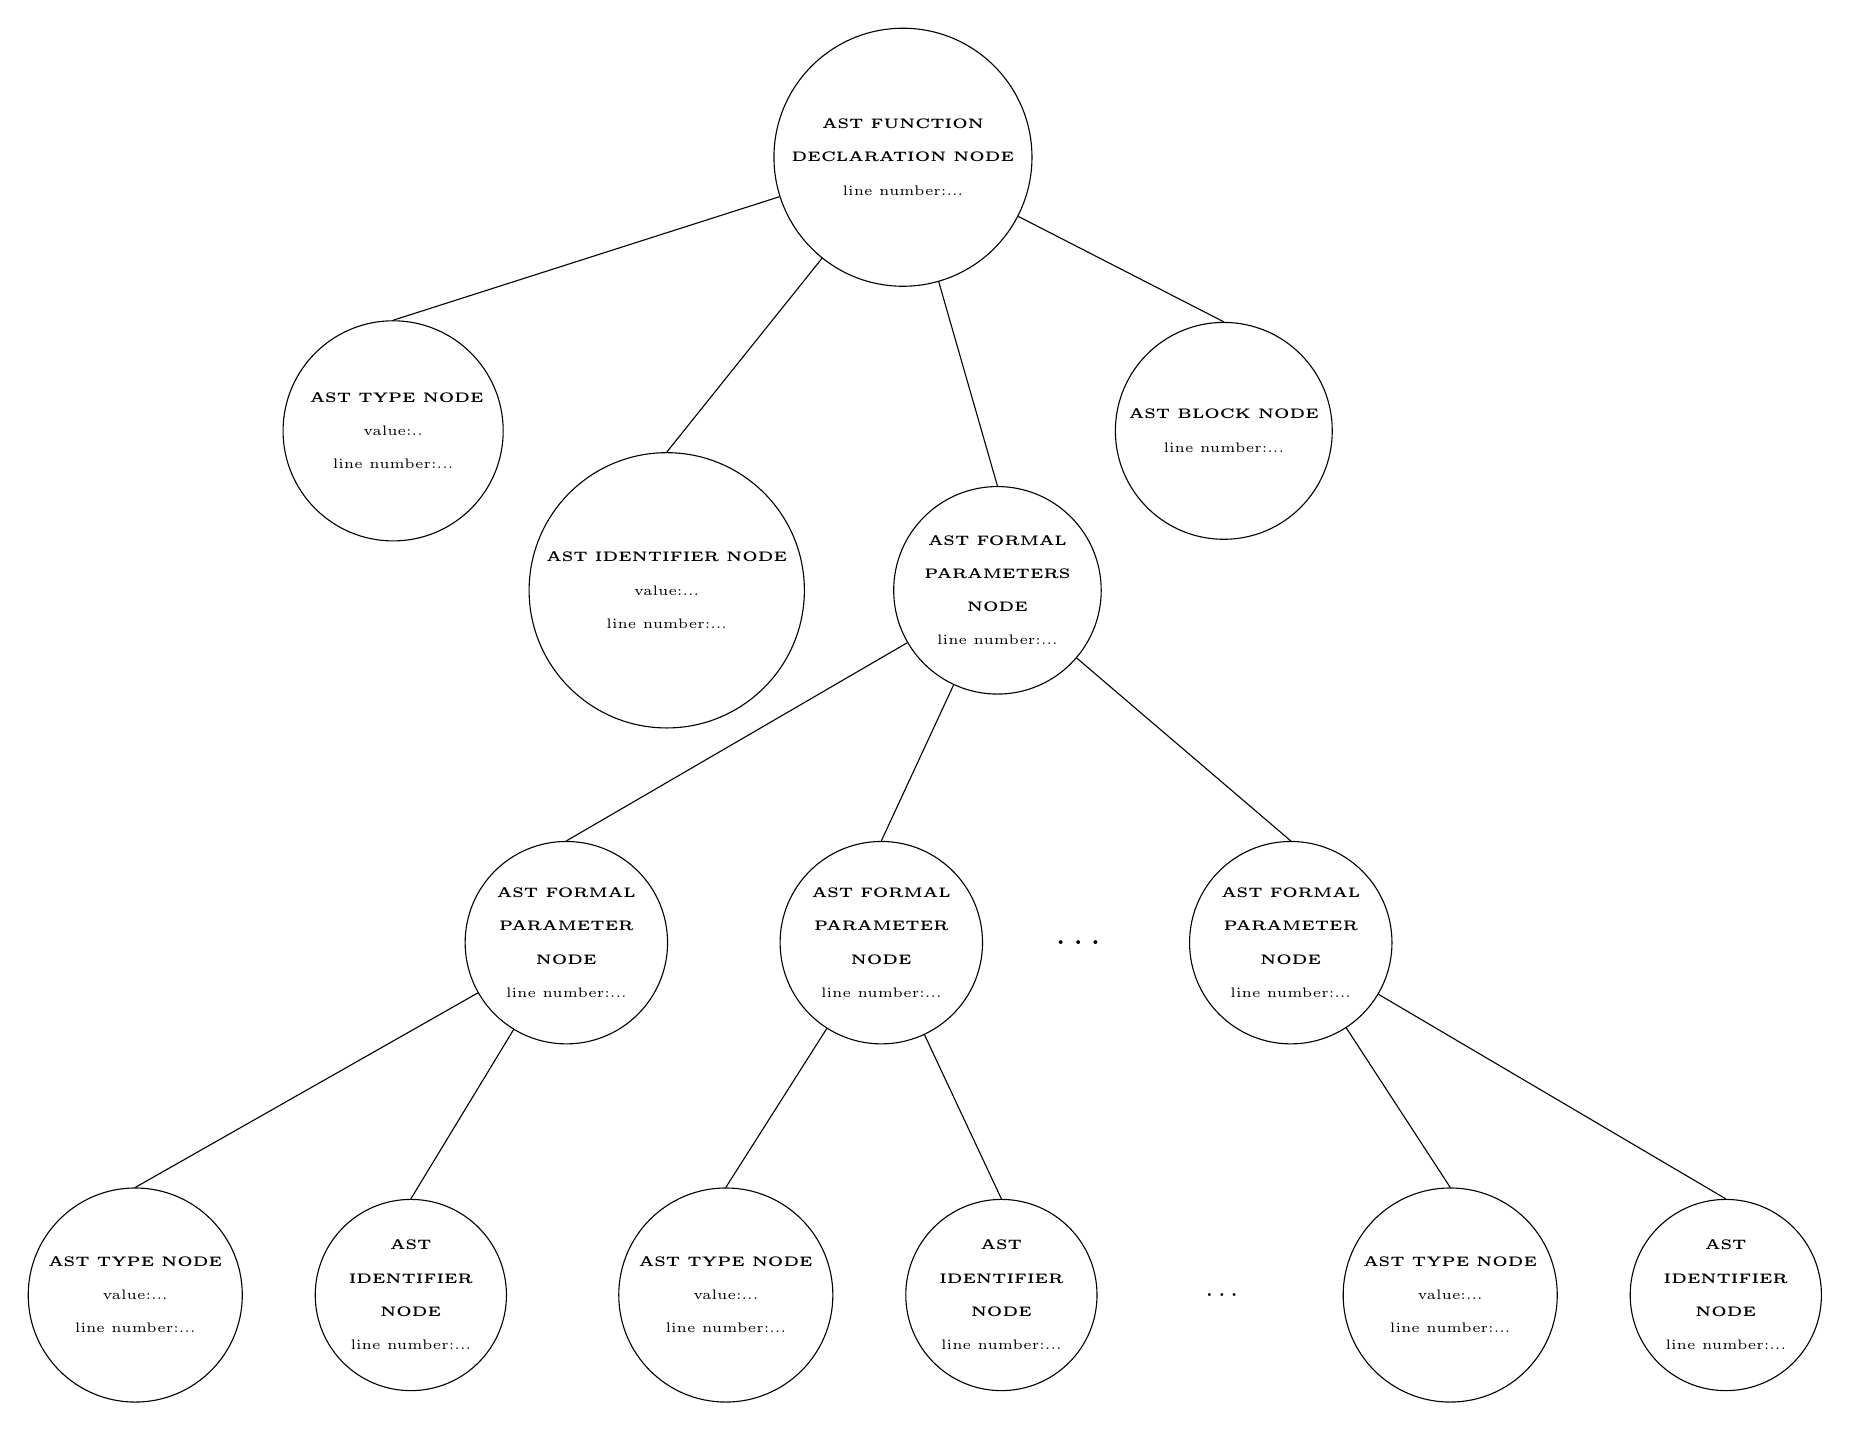
\begin{tikzpicture}[node distance={35mm},main/.style = {draw, circle}] 
			\node[main] (1) [align=center] {\tiny \textbf{AST FUNCTION }\\\tiny \textbf{DECLARATION NODE}\\ \tiny line number:...}; 
			\node[main] (2) [xshift=-4cm,yshift=-1cm,below left of=1,align=center] {\tiny\textbf{ AST TYPE NODE} \\ \tiny value:..\\ \tiny line number:...};
			\node[main] (3) [below  of=1,xshift=-3cm,yshift=-2cm,align=center] {\tiny \textbf{AST IDENTIFIER NODE}\\ \tiny value:...\\ \tiny line number:...};
			\node[main] (4) [xshift=0.7cm,right of=3,align=center] {\tiny \textbf{AST FORMAL} \\\tiny \textbf{PARAMETERS}\\ \tiny \textbf{NODE}\\ \tiny line number:...};
			    
			\node[main] (a) [yshift=-2cm,xshift=-3cm,below left of=4,align=center] {\tiny \textbf{AST FORMAL} \\\tiny \textbf{PARAMETER}\\ \tiny \textbf{NODE}\\ \tiny line number:...};
			\node[main] (ta) [yshift=-2cm,xshift=-3cm,below left of=a,align=center] {\tiny \textbf{AST TYPE NODE}  \\ \tiny value:...\\ \tiny line number:...};
			\node[main] (ia) [right of=ta,align=center] {\tiny \textbf{AST} \\\tiny \textbf{IDENTIFIER}\\ \tiny \textbf{NODE}\\ \tiny line number:...};
			    
			    
			    
			    
			    
			\node[main] (b) [xshift=0.5cm,right of=a,align=center] {\tiny \textbf{AST FORMAL} \\\tiny \textbf{PARAMETER}\\ \tiny
				\textbf{NODE}\\ \tiny line number:...};
			\node[main] (tb) [yshift=-2cm,xshift=0.5cm,below left of=b,align=center] {\tiny \textbf{AST TYPE NODE}  \\ \tiny value:...\\ \tiny line number:...};
			\node[main] (ib) [right of=tb,align=center] {\tiny \textbf{AST} \\\tiny \textbf{IDENTIFIER}\\ \tiny \textbf{NODE}\\ \tiny line number:...};
			\node[] (lb) [xshift=2.8cm,right of=tb,align=center] {\HUGE $\ldots$};
			
			    
			    
			    
			    
			\node[] [xshift=-1cm,right of=b]{\Large$\ldots$};
			\node[main] (c) [xshift=1.7cm,right of=b,align=center] {\tiny \textbf{AST FORMAL} \\\tiny \textbf{PARAMETER}\\ \tiny \textbf{NODE}\\ \tiny line number:...};
			\node[main] (tc) [yshift=-2cm,xshift=4.5cm,below left of=c,align=center] {\tiny \textbf{AST TYPE NODE}  \\ \tiny value:...\\ \tiny line number:...};
			\node[main] (ic) [right of=tc,align=center] {\tiny \textbf{AST} \\\tiny \textbf{IDENTIFIER}\\ \tiny \textbf{NODE}\\ \tiny line number:...};
			    
			\node[main] (5) [xshift=1.6cm,yshift=-1cm,below right of=1,align=center]  {\tiny {\textbf{AST BLOCK NODE}}\\\tiny line number:...}; 
			\draw (1)--(2.north);
			\draw (1)--(3.north);
			\draw (1)--(4.north);
			\draw (4)--(a.north);
			\draw (a)--(ta.north);
			\draw (a)--(ia.north);
			\draw (b)--(tb.north);
			\draw (b)--(ib.north);
			\draw (c)--(tc.north);
			\draw (c)--(ic.north);
			\draw (4)--(b.north);
			\draw (4)--(c.north);
			\draw (1)--(5.north);
		\end{tikzpicture}
	}
	\caption{Statement tree: \textbf{FUNCTION DECLARATION}}
	\label{fig:function declaration tree}
\end{figure}
\begin{lstlisting}[caption=PSEUDOCODE for building a function declaration statement tree (\emph{parseFunctionDeclaration()}),label=listing:func declaration tree]
tree = new Tree(AST_FUNCTION_DECLARATION_NODE,getCurrentToken().lineNumber)
//token that lead to this method should be of type TOK_FN
if(getCurrentToken().type != TOK_FN):
    throw exception unexpected
//get next token (this updates the current token)
Token identifier = getNextToken()
//expect identifier 
Token identifier
if getCurrentToken().type ==TOK_IDENTIFIER
    identifier=getCurrentToken()
else 
    throw exception unexpected
//get next token (this updates the current token)
getNextToken()
//expect (
if(getCurrentToken().type != TOK_LEFT_ROUND_BRACKET):
    throw exception unexpected
//get next token (this updates the current token)
getNextToken()
//expect 0 or more formal parameters
Tree formalParamsSubtree
//if next token is not a right round bracket we have formal paramaters
if(getCurrentToken().type != TOK_RIGHT_ROUND_BRACKET):
    formalParamsSubtree = parseFormalParams()
    //get next token (this updates the current token)
    getNextToken()
//else just add a formal parameters node with no children
else
    formalParamsSubtree = new Tree(AST_FORMAL_PARAMETERS_NODE,getCurrentToken().lineNumber) 
//expect )
if(getCurrentToken().type != TOK_RIGHT_ROUND_BRACKET):
    throw exception unexpected
//get next token (this updates the current token)
getNextToken()
//expect ->
if(getCurrentToken().type != TOK_RIGHT_ARROW):
    throw exception unexpected
 //get next token (this updates the current token)
getNextToken()   
//expect type
Tree typeSubtree = parseType()
//get next token (this updates the current token)
getNextToken()
//expect block 
Tree blockSubtree = parseSubtree()
//add type subtree to function declaration tree
tree.addSubtree(typeSubtree)
//add identifier node to function declartion tree
tree.addChild(AST_IDENTIFIER_NODE,identifier.lexeme,identifier.lineNumber)
//add formal params subtree to function declaration tree
tree.addSubtree(formalParamsSubtree)
//add block subtree to function declaration tree
tree.addSubtree(blockSubtree)
//return function declaration tree
return tree
\end{lstlisting}
Note in PSEUDOCODE shown in listing  \ref{listing:func declaration tree}  their are calls to 3 other parsing methods:
\verb!parseFormalParams()!, \verb!parseType()!, ,\verb!parseBlock()!.  \verb!parseType()! and  \verb!parseBlock()! are described in PSEUDOCODE in listings \ref{listing:type tree} and \ref{listing:block statement tree} respectively.

A diagram of a formal parameter subtree is shown in figure \ref{fig:formal params subtree}.
\begin{figure}[H]
	\centering
	\resizebox{10.5cm}{6cm}{
		\begin{tikzpicture}[node distance={35mm},main/.style = {draw, circle}] 
			\node[main] (4) [xshift=0.7cm,right of=3,align=center] {\tiny \textbf{AST FORMAL} \\\tiny \textbf{PARAMETERS}\\ \tiny \textbf{NODE}\\ \tiny line number:...};
			\node[main] (a) [yshift=-2cm,xshift=-3cm,below left of=4,align=center] {\tiny \textbf{AST FORMAL} \\\tiny \textbf{PARAMETER}\\ \tiny \textbf{NODE}\\ \tiny line number:...};
			\node[main] (ta) [yshift=-2cm,xshift=-3cm,below left of=a,align=center] {\tiny \textbf{AST TYPE NODE}  \\ \tiny value:...\\ \tiny line number:...};
			\node[main] (ia) [right of=ta,align=center] {\tiny \textbf{AST} \\\tiny \textbf{IDENTIFIER}\\ \tiny \textbf{NODE}\\ \tiny line number:...};
			\node[main] (b) [xshift=0.5cm,right of=a,align=center] {\tiny \textbf{AST FORMAL} \\\tiny \textbf{PARAMETER}\\ \tiny
				\textbf{NODE}\\ \tiny line number:...};
			\node[main] (tb) [yshift=-2cm,xshift=0.5cm,below left of=b,align=center] {\tiny \textbf{AST TYPE NODE}  \\ \tiny value:...\\ \tiny line number:...};
			\node[main] (ib) [right of=tb,align=center] {\tiny \textbf{AST} \\\tiny \textbf{IDENTIFIER}\\ \tiny \textbf{NODE}\\ \tiny line number:...};
			\node[] (lb) [xshift=2.8cm,right of=tb,align=center] {\HUGE $\ldots$};
			\node[] [xshift=-1cm,right of=b]{\Large$\ldots$};
			\node[main] (c) [xshift=1.7cm,right of=b,align=center] {\tiny \textbf{AST FORMAL} \\\tiny \textbf{PARAMETER}\\ \tiny \textbf{NODE}\\ \tiny line number:...};
			\node[main] (tc) [yshift=-2cm,xshift=4.5cm,below left of=c,align=center] {\tiny \textbf{AST TYPE NODE}  \\ \tiny value:...\\ \tiny line number:...};
			\node[main] (ic) [right of=tc,align=center] {\tiny \textbf{AST} \\\tiny \textbf{IDENTIFIER}\\ \tiny \textbf{NODE}\\ \tiny line number:...};
			\draw (4)--(a.north);
			\draw (a)--(ta.north);
			\draw (a)--(ia.north);
			\draw (b)--(tb.north);
			\draw (b)--(ib.north);
			\draw (c)--(tc.north);
			\draw (c)--(ic.north);
			\draw (4)--(b.north);
			\draw (4)--(c.north);
		\end{tikzpicture}
	}
	\caption{Formal parameters subtree}
	
	\label{fig:formal params subtree}
\end{figure}
The following logic is formulated using EBNF rules. (see section \ref{sec:ebnf-tinylang-rules}).
\vskip 0.1in    
Formal parameters is a sequence of formal parameter separated by a comma. Each formal parameter has 2 important attributes the identifier and type.
    
The PSEUDOCODE for constructing a formal parameter subtree is given below.
\begin{lstlisting}[caption=PSEUDOCODE for building a formal parameters subtree,label=listing:formal params subtree]
tree = new Tree(AST_FORMAL_PARAMS_NODE,getCurrentToken().lineNumber)
//add formal param
tree.addSubtree(parseFormalParam())
//get next token (this updates the current token)
getNextToken()
//each formal parameter is seperated by a comma
while(getCurrentToken().tokenType==TOK_COMMA)
    //get next token (this updates the current token)
    getNextToken() 
    //parse next formal parameter
    tree.addSubtree(parseFormalParam())
    //get next token (this updates the current token)
    getNextToken() 
//get prev token (this updates the current token)
getPrevToken();
return tree
\end{lstlisting}


Note that in listing \ref{listing:formal params subtree} a call to \verb!parseFormalParam()! is made. Since a formal parameter is made up of 2 important attributes the identifier and type. We parse a formal parameter by parsing through the identifier and type, PSEUDOCODE is given below.
\begin{lstlisting}[caption=PSEUDOCODE for building a formal parameter subtree (\emph{parseFormalParam()}),label=listing:formal param subtree]
tree = new Tree(AST_FORMAL_PARAMETER_NODE,getCurrentToken().lineNumber)
//expect identifier 
if getCurrentToken().type ==TOK_IDENTIFIER
    identifier=getCurrentToken()
//get a hold of identifier node
Token identifier = getCurrentToken();
//get next token (this updates current token)
getNextToken();
//expect :
if getCurrentToken().type ==TOK_COLON
    identifier=getCurrentToken()
//get next token (this updates current token)
getNextToken();
//add type subtree
tree.addSubtree(parseType())
//add identifier
tree.addChild(AST_IDENTIFIER,identifier.lexeme,identifier.lineNumber)
//return tree
return tree
\end{lstlisting}
\textbf{Note} that in listing above, a call to \verb!parseType()! is made. Parsing of a type is discussed in listing \ref{listing:type tree}.






\subsubsection{Block Statement}
\label{sec:block statement tree}
If the current lookahead token is of type \verb!TOK_LEFT_CURLY_BRACKET!, \verb!parseBlock()! is called. 
A block node is equivalent to a program node with the difference that the sequence of statements are enclosed in curly brackets.
\begin{figure}[H]
	\centering
	\resizebox{6cm}{4.5cm}{
		\begin{tikzpicture}[node distance={35mm},main/.style = {draw, circle}] 
			\node[main] (1) [align=center] {AST\\BLOCK\\NODE\\line number:...}; 
			\node[main,regular polygon,regular polygon sides = 3,minimum size=2cm] (2) [xshift=-1cm,yshift=-1cm,below left of=1] {$S_1$};
			\node[main,regular polygon,regular polygon sides = 3,minimum size=2cm] (3) [below  of=1,xshift=-1cm] {$S_2$};
			\node[] (4) [xshift=-2cm,right of=3] {$\ldots$};
			\node[main,regular polygon,regular polygon sides = 3,minimum size=2cm] (5) [yshift=-1cm,below right of=1] {$S_n$};
			\draw (1)--(2.north);
			\draw (1)--(3.north);
			\draw (1)--(5.north);
		\end{tikzpicture}
	}
	\caption{Statement tree: Block is a sequence of statements $S_1,S_2,\ldots,S_n$}
	\label{fig:tinylang block tree}
\end{figure}
\begin{lstlisting}[caption=PSEUDOCODE for building a block tree (\emph{parseBlock()}),label=listing:block statement tree]
tree = new Tree(AST_BLOCK_NODE,getCurrentToken().lineNumber)
//token that lead to this method should be of type {
if(getCurrentToken().type != TOK_LEFT_CURLY_BRACKET):
    throw exception unexpected 
//get next token (this updates current token)
getNextToken()    
//we may have one or more statements block ends using }
while(getCurrentToken().getTokenType()!=TokenType.TOK_RIGHT_CURLY_BRACKET and getCurrentToken().getTokenType()!=TokenType.TOK_EOF ):
    tree.addSubtree(parseStatement())
    getNextToken()

//current token should be }
if(getCurrentToken().type != TOK_LEFT_RIGHT_BRACKET):
    throw exception unexpected 
return tree
\end{lstlisting}



\subsection{Expression Tree(s)}
\label{sec:expression tree building }
An expression tree is a tree where the intermediate nodes correspond to a binary operator and the leave nodes are values to the corresponding binary operator.

\begin{figure}[H]
	\centering
	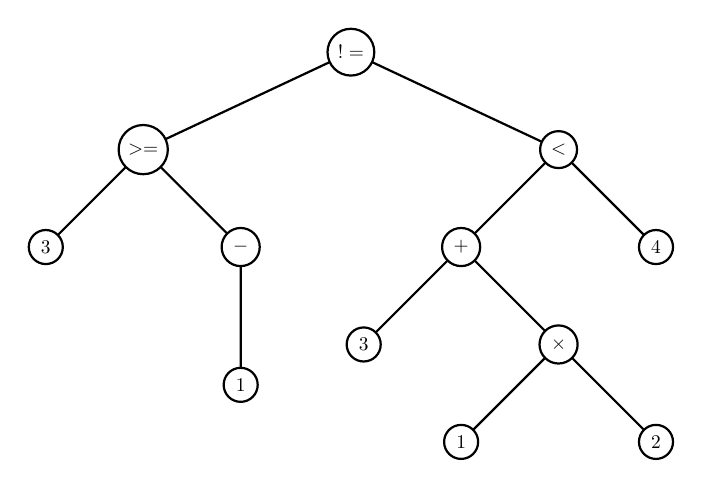
\begin{tikzpicture}[node distance={25mm}, thick, main/.style = {draw, circle},scale=0.15, every node/.style={scale=0.7}]  
		\node[main] (1) {$!=$}; 
		\node[main] (2)[xshift=-2cm,below left of=1] {$>=$}; 
		\node[main] (3)[xshift=2cm,below right of=1]{$<$};
		\node[main] (4)[below right of=2] {$-$}; 
		\node[main] (5)[below of=4]{$1$};
		\node[main] (6)[below left of=3]{$+$};
		\node[main] (7)[below right of=6]{$\times$};
		\node[main] (8)[below right of=3]{$4$};
		\node[main] (9)[below left of=2]{$3$};
		\node[main] (10)[below left of=6]{$3$};
		  
		\node[main] (11)[below left of=7]{$1$};
		\node[main] (12)[below right of=7]{$2$};
		  
		\draw (1)--(2);
		\draw (1)--(3);
		\draw (2)--(4);
		\draw (4)--(5);
		\draw (3)--(6);
		\draw (3)--(8);
		\draw (2)--(9);
		\draw (6)--(7);
		\draw (6)--(10);
		\draw (7)--(11);
		\draw (7)--(12);
		
	\end{tikzpicture}
	\caption{Example of an \textbf{expression tree}}
	\label{fig:example of an expression tree}
\end{figure}
An inorder traversal of the expression tree shown in figure \ref{fig:example of an expression tree} gives us the expression $((3)>=(-1))!=(((3)+((1)\times(2)))<(4))$ which evaluates to true.

As per EBNF rules (see section \ref{sec:ebnf-tinylang-rules}) we parse an expression using the following non terminals:
\verb!<Expression>!, \verb!<SimpleExpression>!, \verb!<Term>! and \verb!<Factor>!.

\subsubsection{<Expression>}
\label{sec:expression tree}
Expression is a sequence of one or more simple expression separated by a relational operator (see section \ref{sec:ebnf-tinylang-rules}). For example suppose we have $se_1 \; relop_1  \; se_2 \;  relop_2  \; \ldots \; relop_{n-1} se_n \equiv  se_1 \; relop_1  \; (se_2 \;  relop_2  \; \ldots  (se_{n-1}\; relop_{n-1} se_n))$
(se denotes simple expression) then a tree representing this expression would look like the following:

\begin{figure}[H]
	\centering
	\resizebox{8.5cm}{6cm}{
		\begin{tikzpicture}[node distance={35mm},main/.style = {draw, circle}] 
			\node[main] (1) [align=center] {\tiny \textbf{AST BINARY}\\ \tiny \textbf{EXPRESSION} \tiny \textbf{NODE} \\ \tiny value:$relop_1$\\ \tiny line number:...}; 
			\node[main,regular polygon,regular polygon sides = 3,minimum size=2cm] (2) [xshift=-2cm,yshift=-1cm,below left of=1,align=center] {$se_1$};
			\node[main] (3) [xshift=1cm,yshift=-1cm,below right of=1,align=center] {\tiny \textbf{AST BINARY}\\ \tiny \textbf{EXPRESSION} \tiny \textbf{NODE} \\ \tiny value:$relop_2$\\ \tiny line number:...};
			\node[main,regular polygon,regular polygon sides = 3,minimum size=2cm] (4) [xshift=-2cm,yshift=-1cm,below left of=3,align=center] {$se_2$};
			
			\node[main] (7) [xshift=2cm,yshift=-1cm,below right of=3,align=center] {\tiny \textbf{AST BINARY}\\ \tiny \textbf{EXPRESSION} \tiny \textbf{NODE} \\ \tiny value:$relop_{n-1}$\\ \tiny line number:...};
			\node [main,regular polygon,regular polygon sides = 3,minimum size=2cm] (8) [xshift=-2cm,yshift=-1cm,below left of=7,align=center] {$se_{n-1}$};
			\node [main,regular polygon,regular polygon sides = 3,minimum size=2cm] (9) [xshift=2cm,yshift=-1cm,below right of=7,align=center] {$se_{n}$};
			\draw (1)--(2.north);
			\draw (1)--(3.north);
			\draw (3)--(4.north);
			\draw (3)--(7.north);
			\draw (7)--(8.north);
			\draw (7)--(9.north);
		\end{tikzpicture}
	}
	\caption{Expression is a sequence of simple expressions separated by an operator of type \emph{TOK\_RELATIONAL\_OP}}
	\label{fig:expression tree 1}
\end{figure}

The tree shown in \ref{fig:expression tree 1} can be defined recursively (note that the right operand has a similar structure).
\begin{itemize}
	\item Base Case: The expression tree is just 1 simple expression.
	      \begin{center}
	      	\resizebox{2cm}{1.5cm}{
	      		\begin{tikzpicture}[node distance={35mm},main/.style = {draw, circle}] 
	      			\node[main,regular polygon,regular polygon sides = 3,minimum size=2cm] (1)  {$se_i$};
	      		\end{tikzpicture}
	      	}
	      \end{center}
	\item Recursive Case:
	      \begin{center}
	      	\resizebox{8.5cm}{5cm}{
	      		\begin{tikzpicture}[node distance={35mm},main/.style = {draw, circle}] 
	      			\node[main] (1) [align=center] {\tiny \textbf{AST BINARY}\\ \tiny \textbf{EXPRESSION} \tiny \textbf{NODE} \\ \tiny value:$relop_1$\\ \tiny line number:...}; 
	      			\node[main,regular polygon,regular polygon sides = 3,minimum size=2cm] (2) [xshift=-2cm,yshift=-1cm,below left of=1,align=center] {$se_1$};
	      			\node[main,regular polygon,regular polygon sides = 3,minimum size=2cm] (3) [xshift=1cm,yshift=-1cm,below right of=1,align=center] {\tiny \textbf{EXPRESSION} \\ \tiny \textbf{TREE}};
	      			\draw (1)--(2.north);
	      			\draw (1)--(3.north);
	      		\end{tikzpicture}
	      	}
	      \end{center}
\end{itemize}

The method of parsing $<Expression>$ and building an expression tree recursively is described in the following PSEUDOCODE.
\begin{lstlisting}[caption=PSEUDOCODE : parsing \emph{<Expression>} and building an expression tree (\emph{parseExpression()})]
// base case
Tree leftOperand = parseSimpleExpression()
//get next token (this updates current token) 
getNextToken()
//if we have a relop run recursive case
if(getCurrentToken().type != TOK_RELATIONAL_OP):
    // build a binary tree value -> lexeme (representing the operator)
    tree = new Tree(AST_BINARY_OPERATOR_NODE,getCurrentToken().lexeme,getCurrentToken().lineNumber)
    //add left operand of binary operator
    tree.addSubtree(leftOperand)
    //recursive step
    tree.addSubtree(parseExpression())
    return tree
return leftOperand
\end{lstlisting}
Note a recursive call is made in line \verb!tree.addSubtree(parseExpression())!. A call to parse a simple expression tree is also made via \verb!parseSimpleExpression()!. Parsing of a simple expression is discussed in \ref{sec:parse simple expresion}




\subsubsection{<SimpleExpression>}
\label{sec:parse simple expresion}
Simple Expression is a sequence of one or more simple expression separated by a additive operator (see section \ref{sec:ebnf-tinylang-rules}). For example suppose we have $term_1 \; additiveOp_1  \; term_2 \;  additiveOp_2  \; \ldots \; additiveOp_{n-1} term_n \equiv  term_1 \; additiveOp_1  \; (term_2 \;  additiveOp_2  \; \ldots  (term_{n-1}\; additiveOp_{n-1} term_n))$



A simple expression can be built recursively similar to as discussed in section \ref{sec:expression tree building } where 
\begin{itemize}
	\item Base Case: The simple expression tree is just 1 simple expression.
	      \begin{center}
	      	\resizebox{2cm}{1.5cm}{
	      		\begin{tikzpicture}[node distance={35mm},main/.style = {draw, circle}] 
	      			\node[main,regular polygon,regular polygon sides = 3,minimum size=2cm] (1)  {$term_i$};
	      		\end{tikzpicture}
	      	}
	      \end{center}
	\item Recursive Case:
	      \begin{center}
	      	\resizebox{9.3cm}{5cm}{
	      		\begin{tikzpicture}[node distance={35mm},main/.style = {draw, circle}] 
	      			\node[main] (1) [align=center] {\tiny \textbf{AST BINARY}\\ \tiny \textbf{EXPRESSION} \tiny \textbf{NODE} \\ \tiny value:$additiveOp_1$\\ \tiny line number:...}; 
	      			\node[main,regular polygon,regular polygon sides = 3,minimum size=2cm] (2) [xshift=-2cm,yshift=-1cm,below left of=1,align=center] {$term_1$};
	      			\node[main,regular polygon,regular polygon sides = 3,minimum size=2cm] (3) [xshift=1cm,yshift=-1cm,below right of=1,align=center] {\tiny \textbf{SIMPLE} \\ \tiny \textbf{EXPRESSION}\\ \tiny \textbf{TREE}};
	      			\draw (1)--(2.north);
	      			\draw (1)--(3.north);
	      		\end{tikzpicture}
	      	}
	      \end{center}
	      
\end{itemize}



The method of parsing $<SimpleExpression>$ and building an expression tree recursively is described in the following pseudocode.
\begin{lstlisting}[caption=parsing \emph{<SimpleExpression>} and building an expression tree (\emph{parseSimpleExpression()})]
// base case
Tree leftOperand = parseTerm()
//get next token (this updates current token) 
getNextToken()
//if we have a relop run recursive case
if(getCurrentToken().type != TOK_ADDITIVE_OP):
    // build a binary tree value -> lexeme (representing the operator)
    tree = new Tree(AST_BINARY_OPERATOR_NODE,getCurrentToken().lexeme,getCurrentToken().lineNumber)
    //add left operand of binary operator
    tree.addSubtree(leftOperand)
    //recursive step
    tree.addSubtree(parseSimpleExpression())
    return tree
return leftOperand
\end{lstlisting}
Note a recursive call is made in line \verb!tree.addSubtree(parseExpression())!. A call to parse a term is also made via \verb!parseTerm()!. Parsing of a term is discussed in \ref{sec:parse term expresion}.

\subsubsection{<Term>}
\label{sec:parse term expresion}
Term  is a sequence of one or more  factors separated by a multiplicative operator (see section \ref{sec:ebnf-tinylang-rules}). For example suppose we have $factor_1 \; multiplicativeOp_1  \; term_2 \;  multiplicativeOp_2  \; \ldots \; multiplicativeOp_{n-1} term_n \equiv  factor _1 \; additiveOp_1  \; (factor_2 \;  multiplicativeOp_2  \; \ldots  (factor_{n-1}\; multiplicativeOp_{n-1} factor_n))$



A term  can be built recursively similar to as discussed in sections \ref{sec:expression tree building } and \ref{sec:parse simple expresion} where 
\begin{itemize}
	\item Base Case: The simple expression tree is just 1 simple expression.
	      \begin{center}
	      	\resizebox{2cm}{1.5cm}{
	      		\begin{tikzpicture}[node distance={35mm},main/.style = {draw, circle}] 
	      			\node[main,regular polygon,regular polygon sides = 3,minimum size=2cm] (1)  {$factor_i$};
	      		\end{tikzpicture}
	      	}
	      \end{center}
	\item Recursive Case:
	      \begin{center}
	      	\resizebox{9.3cm}{5cm}{
	      		\begin{tikzpicture}[node distance={35mm},main/.style = {draw, circle}] 
	      			\node[main] (1) [align=center] {\tiny \textbf{AST BINARY}\\ \tiny \textbf{EXPRESSION} \tiny \textbf{NODE} \\ \tiny value:$multiplicativeOp_1$\\ \tiny line number:...}; 
	      			\node[main,regular polygon,regular polygon sides = 3,minimum size=2cm] (2) [xshift=-2cm,yshift=-1cm,below left of=1,align=center] {$factor_1$};
	      			\node[main,regular polygon,regular polygon sides = 3,minimum size=2cm] (3) [xshift=1cm,yshift=-1cm,below right of=1,align=center] {\tiny \textbf{SIMPLE} \\ \tiny \textbf{EXPRESSION}\\ \tiny \textbf{TREE}};
	      			\draw (1)--(2.north);
	      			\draw (1)--(3.north);
	      		\end{tikzpicture}
	      	}
	      \end{center}
	      
\end{itemize}



The method of parsing $<Term>$ and building an expression tree recursively is described in the following pseudocode.
\begin{lstlisting}[caption=parsing \emph{<Term>} and building an expression tree (\emph{parseTerm()})]
// base case
Tree leftOperand = parseFactor()
//get next token (this updates current token) 
getNextToken()
//if we have a relop run recursive case
if(getCurrentToken().type != TOK_MULTIPLICATIVE_OP):
    // build a binary tree value -> lexeme (representing the operator)
    tree = new Tree(AST_BINARY_OPERATOR_NODE,getCurrentToken().lexeme,getCurrentToken().lineNumber)
    //add left operand of binary operator
    tree.addSubtree(leftOperand)
    //recursive step
    tree.addSubtree(parseFactor())
    return tree
return leftOperand
\end{lstlisting}
Note a recursive call is made in line \verb!tree.addSubtree(parseExpression())!. A call to parse a factor is also made via \verb!parseFactor()!. Parsing of a factor is discussed in \ref{sec:parse factor expression}

\subsubsection{<Factor>}
\label{sec:parse factor expression}
A factor represents an operand of the binary operator. Now an operand may take different forms (see section \ref{sec:ebnf-tinylang-rules}) namely:
\begin{itemize}
	\item Literal : A constant value e.g. $1$, $true$, $5.3$,$'a'$ etc.
	\item Identifier : Representing a variable. The operand operates on the value of that variable.
	\item FunctionCall : A call to a function that is expected to return some value. That value is used as the operand.
	\item SubExpression : The operand might be a value return by another expression.
	\item Unary  : A unary operator followed by an expression e.g. +5,  -(2+3.2), not 5>3 etc.
\end{itemize}
We use a 1 look ahead token to deterministically decide what the type of the operand is and parse accordingly.
\vskip 0.1in
The logic of \verb!parseFactor()! is given by the following list of cases.

\textbf{If the current lookahead token is of type:}
\begin{itemize}
	\item  \verb!TOK_BOOLEAN_LITERAL! return the following node
	      \begin{center}
	      	\resizebox{2.5cm}{2.3cm}{
	      		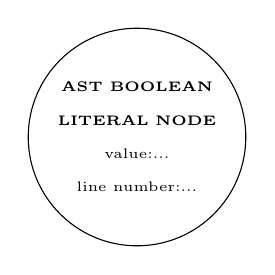
\begin{tikzpicture}[node distance={35mm},main/.style = {draw, circle}] 
	      			\node[main] (1) [align=center] {\tiny \textbf{AST BOOLEAN} \\ \tiny \textbf{LITERAL}  \textbf{NODE} \\ \tiny value:... \\ \tiny line number:...};
	      		\end{tikzpicture}
	      	}
	      \end{center}
	      \begin{itemize}
	      	\item Return similar nodes on token types \verb!TOK_INT_LITERAL!, \verb!TOK_FLOAT_LITERAL! and \verb!TOK_CHAR_LITERAL!
	      \end{itemize}
	\item \verb!TOK_IDENTIFIER!. This leads to possible cases. The operand is either an identifier or a function call. We keep the implementation deterministic (k=1) by checking if the next token is a left round bracket.
	      \begin{itemize}
	      	\item If next token is a left round bracket we deduce that the operand is a function call and we return the subtree produced by parsing a function call (\verb!parseFunctionCall()!) (see section \ref{sec:function call factor} for discussion of function call tree)
	      	\item Otherwise we deduce that the operand is just an identifier and return the following node:
	      	      \begin{center}
	      	      	\resizebox{2.5cm}{2.3cm}{
	      	      		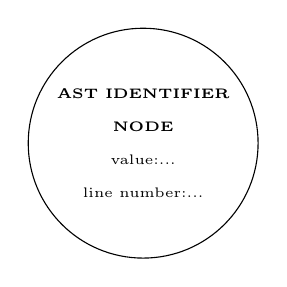
\begin{tikzpicture}[node distance={35mm},main/.style = {draw, circle}] 
	      	      			\node[main] (1) [align=center] {\tiny \textbf{AST IDENTIFIER} \\ \tiny  \textbf{NODE} \\ \tiny value:... \\ \tiny line number:...};
	      	      		\end{tikzpicture}
	      	      	}
	      	      \end{center}
	      	\item \verb!TOK_LEFT_ROUND_BRACKET! then return the tree produced by parsing a sub expression (\verb!parseSubExpression()!) (see section \ref{sec:sub expression factor} for discussion of sub expression tree)
	      	\item \verb!TOK_ADDITIVE_OP! or \verb!TOK_NOT! then return the tree produced by parsing an unary expression (\verb!parseUnary()!) (see section \ref{sec:unary expression factor} for discussion of unary tree)
	      	\item for other tokens \verb!throw exception unexpected!
	      \end{itemize}
\end{itemize}


\paragraph{Factor : Unary Expression}

\label{sec:unary expression factor}
\begin{figure}[H]
	\centering
	\begin{tikzpicture}[node distance={35mm},main/.style = {draw, circle}] 
		\node[main] (1) [align=center] {\tiny \textbf{AST UNARY}\\ \tiny \textbf{EXPRESSION} \tiny \textbf{NODE} \\ \tiny value:$+$ or $-$ or $not$\\ \tiny line number:...}; 
		            
		\node[main,regular polygon,regular polygon sides = 3,minimum size=2cm] (3) [yshift=-2cm,below of=1,align=center] {\tiny \textbf{EXPRESSION}\\ \tiny \textbf{TREE}};
		\draw (1)--(3.north);
	\end{tikzpicture}
	\caption{\textbf{Unary expression tree}}
	\label{fig:unary expression building}
\end{figure}

Building of an expression tree is discussed in section \ref{sec:expression tree building }.


While parsing a unary expression we check for unary operators $+$, $-$ and $not$ and construct the unary node accordingly. The PSEUDOCECODE of given below.
\begin{lstlisting}[caption=PSEUDOCODE for building a \textbf{unary expression tree} (\emph{parseUnary()})]
//an additive op or not led to this parsing method 
if(getCurrentToken ().type != TOK_ADDITIVE_OP and getCurrentToken().type != TOK_NOT):
    throw exception unexpected
tree = new Tree( AST_BLOCK_NODE ,getCurrentToken().lexeme, getCurrentToken().lineNumber )
//get next token (this updates current token )
getNextToken ()
//add expression subtree
tree.addSubtree(parseExpression())
return tree
\end{lstlisting}

\paragraph{Factor :Sub Expression}
\label{sec:sub expression factor}

A sub expression is an expression in its own right. We get  hold on the value returned by a sub-expression to use it in other expression by enclosing in its bracket.

Since a sub expression is an expression the tree return by sub expression is an expression tree as described in section \ref{sec:expression tree building }.


When parsing a sub expression we check for a left round bracket we parse an expression and then we check for a right bracket. The pseudocode is given below.
\begin{lstlisting}[caption=PSEUDOCODE for (\emph{parseSubExpression()})]
//an left round bracket led to this parsing method 
if(getCurrentToken ().type != TOK_LEFT_ROUND_BRACKET):
    throw exception unexpected
//get next token(this updates current token)
tree = parseExpression()
//get next token 
getNextToken();
//we expect a right round bracket
if(getCurrentToken().type=TOK_RIGHT_ROUND_BRACKET)
    throw exception unexpected
return tree
\end{lstlisting}

\paragraph{Factor : Function Call}
\label{sec:function call factor}
A function call tree is similar to function declaration tree as described in section \ref{sec:function declaration statement}. We call a function without specifying its type  and block of statements (reference to actual declaration) hence a function call tree need not have a type child and block child. 
But instead of formal parameters subtree we have an actual parameters subtree whose children are expression tree.
\begin{figure}[H]
	\centering
	\resizebox{11.9cm}{9.9cm}{
		\begin{tikzpicture}[node distance={35mm},main/.style = {draw, circle}] 
			\node[main] (1) [align=center] {\tiny \textbf{AST FUNCTION }\\\tiny \textbf{CALL NODE}\\ \tiny line number:...}; 
			
			\node[main] (3) [below  of=1,xshift=-3cm,yshift=-2cm,align=center] {\tiny \textbf{AST IDENTIFIER NODE}\\ \tiny value:...\\ \tiny line number:...};
			\node[main] (4) [xshift=0.7cm,right of=3,align=center] {\tiny \textbf{AST ACTUAL} \\\tiny \textbf{PARAMETERS}\\ \tiny \textbf{NODE}\\ \tiny line number:...};
			    
			
			
			    
			    
			    
			
			
			\node[main,regular polygon,regular polygon sides = 3,minimum size=2cm] (c) [yshift=-2.8cm,xshift=1.7cm,right of=b,align=center] {\tiny \textbf{EXPRESSION} \\\tiny \textbf{TREE} };
			
			    
			\node[] [left of=c] (l) {\Large$\ldots$};
			    
			    
			\node[main,regular polygon,regular polygon sides = 3,minimum size=2cm] (b) [left  of=l ,align=center] {\tiny \textbf{EXPRESSION} \\\tiny \textbf{TREE} };
			
			\node[main,regular polygon,regular polygon sides = 3,minimum size=2cm] (a) [xshift=-2cm,left of=b,align=center] {\tiny \textbf{EXPRESSION} \\\tiny \textbf{TREE} };
			    
			
			
			\draw (1)--(3.north);
			\draw (1)--(4.north);
			\draw (4)--(a.north);
			\draw (4)--(b.north);
			\draw (4)--(c.north);
		\end{tikzpicture}
	}
	\caption{Factor tree: \textbf{FUNCTION CALL}}
	\label{fig:function call tree}
\end{figure}

When parsing a function call factor we check if we have an identifier (the lookahead token that lead to parsing a function call factor) , for brackets enclosing the actual parameters. If we have no parameters the actual parameter node has no children. 

The PSEUDOCODE  is given below.

\begin{lstlisting}[caption=PSEUDOCODE for building a function call expression tree]
tree = new Tree( AST_FUNCTION_CALL_NODE , getCurrentToken().lineNumber )
// token that lead to this method should be of type identifier
if( getCurrentToken ().type != TOK_IDENTIFIER ):
    throw exception unexpected
//add identifier node
tree.addChild(AST_IDENTIFIER_NODE,getCurrentToken().lexeme,getCurrentToken().lineNumber)
// get next token (this updates current token)
getNextToken ()
// next token should be of type (
if(getCurrentToken ().type != TOK_LEFT_ROUND_BRACKET ):
    throw exception unexpected
// get next token (this updates current token)
getNextToken ()
//if the next token is not a round bracket -> we should have one or more actual parameters
if(getCurrentToken ().type != TOK_RIGHT_ROUND_BRACKET ):
    tree.addSubtree(parseActualParams())
    // get next token (this updates current token)
    getNextToken()
//else we add a parameter node with no children
else
    tree.addChild(AST_ACTUAL_PARAMETER_NODE,getCurrenToken().lexeme.getCurrentToken().linenumber)
// get next token (this updates current token)
getNextToken ()
//expect right round bracket
if(getCurrentToken ().type != TOK_RIGHT_ROUND_BRACKET):
    throw exception unexpected
//return tree
return tree
\end{lstlisting}
Note that in the listing above a call to parseActualParameters() is made when we have \textbf{1 or more actual parameters}. An actual parameters tree consists of an actual parameter node with expression subtrees as shown in figure \ref{fig:function call tree}. To parse actual parameters we need to parse 1 or more expression (see section \ref{sec:expression tree building }). 
The PSEUDOCODE of parsing actual parameters is given below /
\begin{lstlisting}[caption=parsing 1 or more actual parameters (\emph{parseActualParams()})]
Tree tree = new TinyLangAst(AST_ACTUAL_PARAMETERS,getCurrentToken().lineNumber)
//add expression subtree
tree addSubtree(parseExpression)
//get next token (this updates current token)
getNextToken()
//we start checking if we have commas since this implies that we have more actual paremeters
while(getCurrenToken().type==TOK_COMMA and getCurrenToken().type!=TOK_EOF):
    //get next token (this updates current token)
    getNextToken()
    //add next expression subtree
    actualParamsTree.addSubtree(parseExpression())
    //get next token (this updates current token)
    getNextToken()
//move back one token (this updates current token)
getPrevToken()
return tree
\end{lstlisting}

\section{Parse tree of a sample tinylang program}

Consider the following tinylang program.
\begin{lstlisting}[caption=a tinylang program,label=listing:tinylangast]
fn Sq (x:float) −> float {
    return x*x ;
}
print Sq(5+2);
\end{lstlisting}
Using the recursive descent parse described using the the methods above starting from \verb!parseTinyLangProgram()! we generate the following AST
\begin{figure}[H]
	\centering
	\resizebox{14.9cm}{15cm}{
		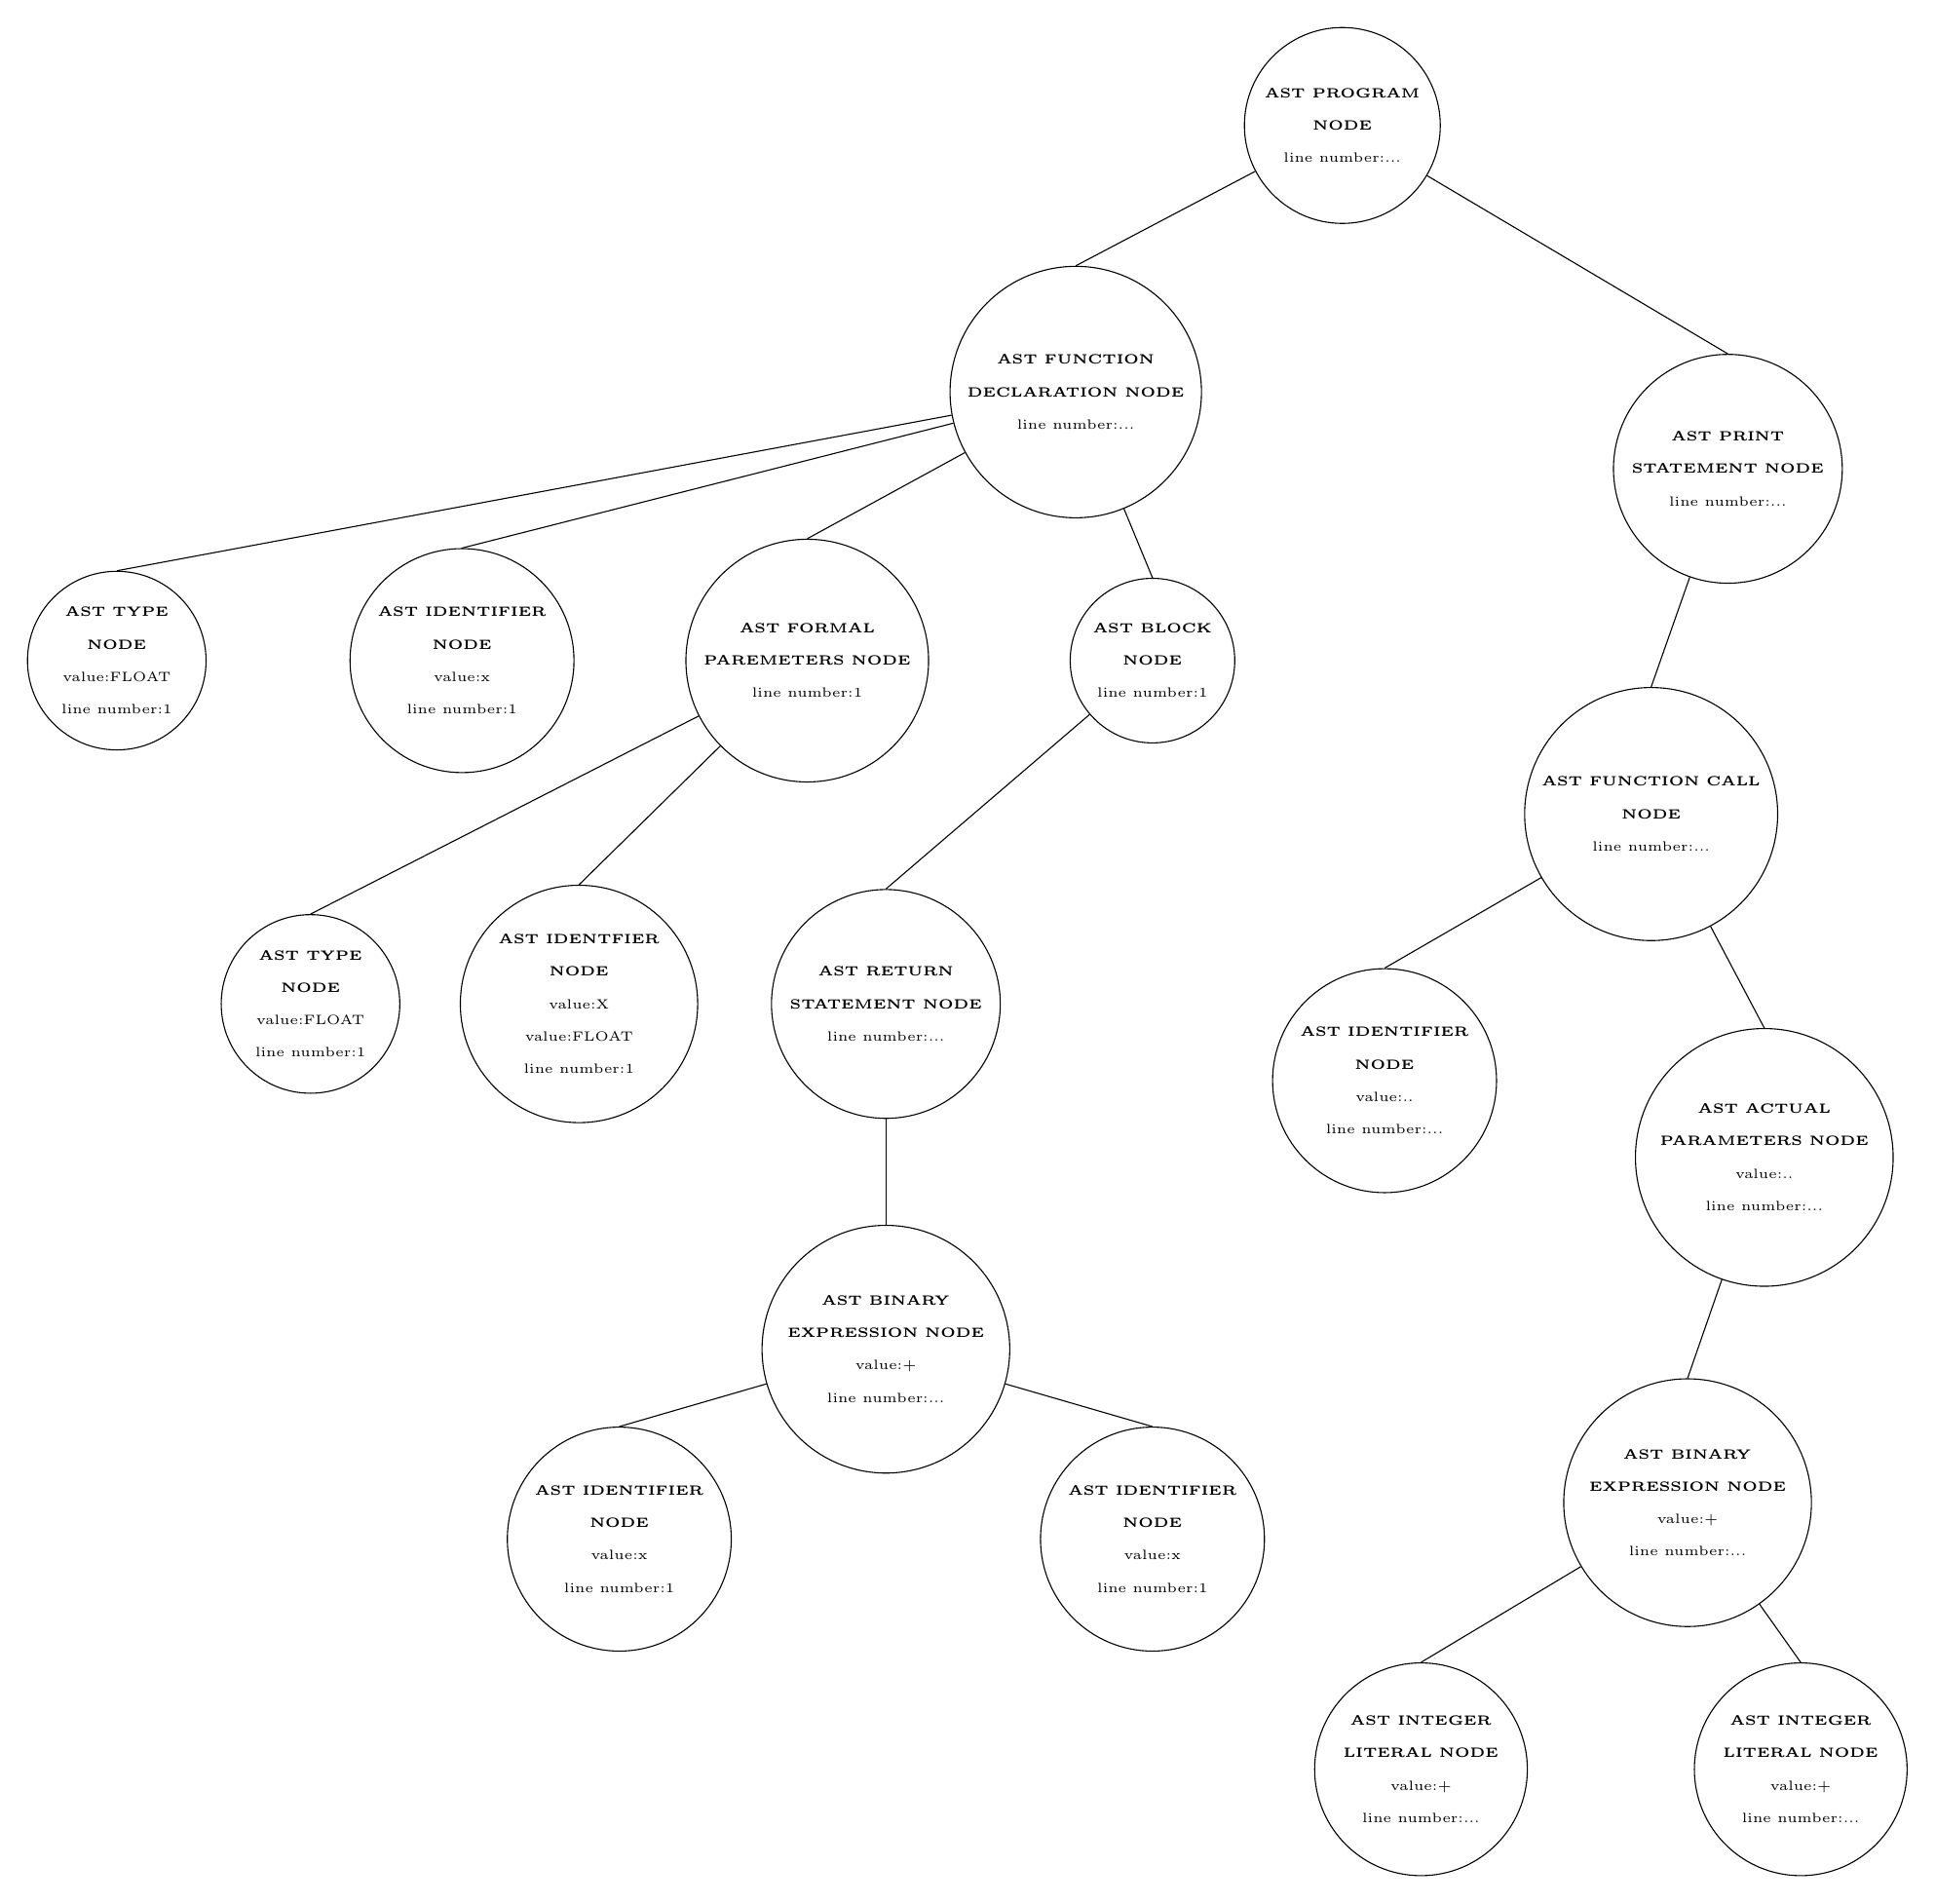
\begin{tikzpicture}[node distance={35mm},main/.style = {draw, circle}] 
			\node[main] (1) [align=center] {\tiny \textbf{AST PROGRAM}\\\tiny \textbf{NODE}\\ \tiny line number:...}; 
			
			\node[main] (3) [yshift=-1cm,xshift=-1cm,below left of=1,align=center] {\tiny \textbf{AST FUNCTION}\\\tiny \textbf{DECLARATION NODE}\\ \tiny line number:...}; 
			          
			      
			\node[main] (5) [xshift=1cm,below of=3,align=center] {\tiny \textbf{AST BLOCK}\\\tiny \textbf{NODE}\\ \tiny line number:1}; 
			\node[main] (6) [xshift=-1cm,left of=5,align=center] {\tiny \textbf{AST FORMAL}\\\tiny \textbf{PAREMETERS NODE}\\ \tiny line number:1}; 
			\node[main] (7) [xshift=-1cm,left of=6,align=center] {\tiny \textbf{AST IDENTIFIER}\\\tiny \textbf{NODE}\\ \tiny value:x\\ \tiny line number:1}; 
			\node[main] (8) [xshift=-1cm,left of=7,align=center] {\tiny \textbf{AST TYPE}\\\tiny \textbf{NODE}\\ \tiny value:FLOAT\\ \tiny line number:1}; 
			          
			\node[main] (10) [xshift=6cm,yshift=-1cm,xshift=-1cm, right of=3,align=center] {\tiny \textbf{AST PRINT}\\\tiny \textbf{STATEMENT NODE}\\ \tiny line number:...}; 
			          
			\node[main] (11) [yshift=-1cm,xshift=-1cm,below of=10,align=center] {\tiny \textbf{AST FUNCTION CALL}\\\tiny \textbf{NODE} \\ \tiny line number:...}; 
			          
			\node[main] (12) [yshift=-1cm,xshift=-1cm,below left of=11,align=center] {\tiny \textbf{AST IDENTIFIER }\\\tiny \textbf{NODE}  \\ \tiny value:..\\ \tiny line number:...}; 
			          
			\node[main] (13) [yshift=-2cm,xshift=-1cm,below right of=11,align=center] {\tiny \textbf{AST ACTUAL }\\\tiny \textbf{PARAMETERS NODE}  \\ \tiny value:..\\ \tiny line number:...}; 
			          
			          
			\node[main] (14) [yshift=-1cm,xshift=-1cm,below of=13,align=center] {\tiny \textbf{AST BINARY}\\\tiny \textbf{EXPRESSION NODE}\\ \tiny value:+\\ \tiny line number:...}; 
			
			
			\node[main] (15) [yshift=-1cm,xshift=-1cm,below left of=14,align=center] {\tiny \textbf{AST INTEGER}\\\tiny \textbf{LITERAL NODE}\\ \tiny value:+\\ \tiny line number:...}; 
			\node[main] (16) [yshift=-1cm,xshift=-1cm,below right of=14,align=center] {\tiny \textbf{AST INTEGER}\\\tiny \textbf{LITERAL NODE}\\ \tiny value:+\\ \tiny line number:...}; 
			           
			           
			\node[main] (17) [yshift=-2cm,xshift=-1cm,below left of=5,align=center] {\tiny \textbf{AST RETURN}\\\tiny \textbf{STATEMENT NODE}\\ \tiny line number:...};
			              
			\node[main] (18) [yshift=-1cm,below of=17,align=center] {\tiny \textbf{AST BINARY}\\\tiny \textbf{EXPRESSION NODE}\\ \tiny value:+\\ \tiny line number:...}; 
			               
			\node[main] (19) [xshift=-4cm,left of=17,align=center] {\tiny \textbf{AST TYPE}\\\tiny \textbf{NODE}\\ \tiny value:FLOAT\\ \tiny line number:1}; 
			          
			      
			\node[main] (20) [xshift=-1cm,below left of=18,align=center] {\tiny \textbf{AST IDENTIFIER}\\\tiny \textbf{NODE}\\ \tiny value:x\\ \tiny line number:1}; 
			               
			\node[main] (21) [xshift=1cm,below right of=18,align=center] {\tiny \textbf{AST IDENTIFIER}\\\tiny \textbf{NODE}\\ \tiny value:x\\ \tiny line number:1}; 
			             
			\node[main] (22) [xshift=0cm,right of=19,align=center] {\tiny \textbf{AST IDENTFIER}\\\tiny \textbf{NODE}\\ \tiny value:X\\ \tiny value:FLOAT\\ \tiny line number:1}; 
			          
			               
			\draw (1)--(10.north);
			\draw (1)--(3.north);
			\draw (3)--(5.north);
			\draw (3)--(6.north);
			\draw (3)--(7.north);
			\draw (3)--(8.north);
			\draw (10)--(11.north);
			\draw (11)--(12.north);
			\draw (11)--(13.north);
			\draw (13)--(14.north);
			\draw (14)--(15.north);
			\draw (14)--(16.north);
			\draw (5)--(17.north);
			\draw (6)--(19.north);
			\draw (6)--(22.north);
			
			\draw (17)--(18.north);
			
			\draw (18)--(20.north);
			\draw (18)--(21.north);
			
		\end{tikzpicture}
	}
	
	\caption{AST generated after parsing program (listing \ref{listing:tinylangast})}
	\label{fig:tiny-lang-ast}
\end{figure}


\section{Implementation in Java}
\begin{itemize}
	\item The  implementation of a general AST (see section \ref{sec:design of an ast}), and the enum constants (see listing \ref{listing:enum nodetype})  used to indicate the the type of subtree is given in listings \ref{listing:tree class implementation} and 
	      \ref{listing:tiny lang node type implementation} respectively.
	\item The implementation of parsing methods discussed in section \ref{sec:recursive descent}
	      is given in listing \ref{listing:rescursive descent parser implementation}.
\end{itemize}
\section{Testing}
\textbf{We test a program that has a number of  syntax errors and fix it.}
\begin{lstlisting}[basicstyle=\tiny,caption=Program 3]
//a function must always return
let x bool=false;
fn forLoop()->bool{
	for(let i:int=1;i<=10;i=i+1){
		print i;
	}
	return true;
}
/*
a statement cannot be a function call (see EBNF)
 we assign an identifier bool x
*/
bool=forLoop();
if(x==(true) {print 'T';} else {print 'F';}
\end{lstlisting}
\begin{itemize}
	\item When executing we get an exception message that we have a missing colon in line 2.
	      \begin{figure}[H]
	      	\centering
	      	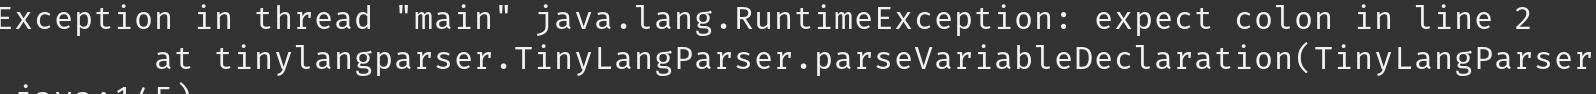
\includegraphics[scale=0.6]{Task2/image/error1.png}
	      	\caption{Exception 1}
	      	\label{fig:Exception 1}
	      \end{figure}
	          
	\item After we add the colon (i.e.
	      \verb!let x bool=false; -> let x : bool=false;!). We execute once again and we get that we have an error indicating that we except a semicolon at line 6.
	      \begin{figure}[H]
	      	\centering
	      	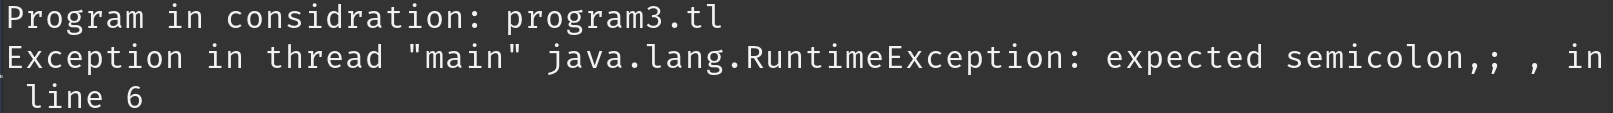
\includegraphics[scale=0.6]{Task2/image/error2.png}
	      	\caption{Exception 2}
	      	\label{fig:Exception 2}
	      \end{figure}
	          
	\item After we add the semicolon (i.e.
	      \verb!print i -> print i;!). We execute once again and we get that we have an error in line 13 indicating that no statement can begin with bool.
	      \begin{figure}[H]
	      	\centering
	      	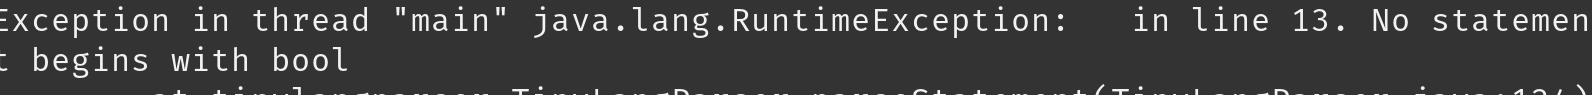
\includegraphics[scale=0.8]{Task2/image/error3.png}
	      	\caption{Exception 3}
	      	\label{fig:Exception 3}
	      \end{figure}
	\item After fixing the error (i.e.
	      \verb!bool=-forLoop(); -> x=forLoop();!). We execute once again and we get the following error.
	      \begin{figure}[H]
	      	\centering
	      	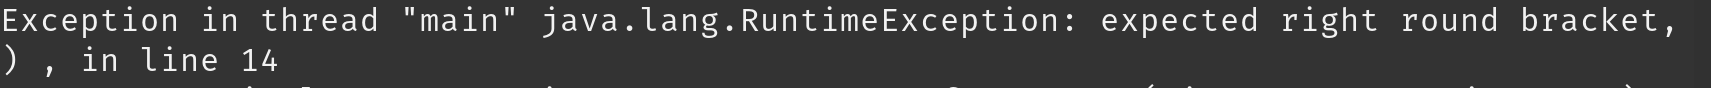
\includegraphics[scale=0.8]{Task2/image/error4.png}
	      	\caption{Exception 4}
	      	\label{fig:Exception 4}
	      \end{figure}
	          
	\item After fixing the error i.e.
	          
	      (\verb!if(x=true){...} else {...} ->! \verb!if(x=true)){...} else {...}!).  \textbf{We get no errors}
	      \begin{figure}[H]
	      	\centering
	      	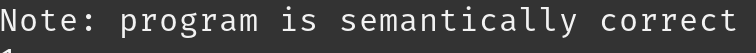
\includegraphics[scale=0.9]{Task2/image/pass.png}
	      	\caption{Success}
	      	\label{fig:succes parse test}
	      \end{figure}
	      Note figure \ref{fig:succes parse test} also implies that the program is semantically correct, this notion is discussed in Task 4.
\end{itemize}